%\input{preamble}
%
%\title{\textsc{Probability Theory and Random Processes (MA225)}}
%\subtitle{\textsc{Lecture Slides}\\ Lecture 22 (September 30, 2019) }
%\author{}
%\date{}


\documentclass[10pt]{beamer} %
\usetheme{CambridgeUS}
% \usecolortheme{seahorse}
\usecolortheme{orchid}
% \usepackage[latin1]{inputenc}
\usefonttheme{professionalfonts}
\usepackage{times}
%\usepackage{tikz}
\usepackage{amsmath}
\usepackage{verbatim}
\usepackage{graphicx}
\usepackage{multicol}
%\usetikzlibrary{arrows,shapes}
\setlength{\tabcolsep}{20pt}
\renewcommand{\arraystretch}{1.5}

\usepackage{amsmath,amssymb,amsfonts}
\usepackage{hyperref}
\usepackage{textcomp}
\usepackage[english]{babel}
\usepackage{times}
% \usepackage[T1]{fontenc}

\usepackage{xcolor}
\usepackage{color, colortbl}
\usepackage{multirow}

%\usepackage{beamerthemesplit}
%\usetheme{Warsaw}
\setbeamertemplate{footline}[frame number]
%\usefonttheme{structurebold}
%\usefonttheme[onlymath]{serif}
%\usefonttheme{serif}
\usepackage{pgf,pgfarrows,pgfnodes,pgfautomata,pgfheaps,pgfshade}
\usepackage{amsmath,amssymb}
% \usepackage{inputenc}
%\usepackage[latin1]{inputenc}
\usepackage[english]{babel}
\usepackage{times}
\usepackage{hyperref}
\usepackage{colortbl}
\usepackage{helvet}
\usepackage{booktabs}
\usepackage{multirow}

\usepackage{tikz}
\usetikzlibrary{arrows,shapes,trees, positioning}
\usepackage{graphics}
\usepackage{color}

\pgfdeclarelayer{background}
\pgfdeclarelayer{foreground}
\pgfsetlayers{background,main,foreground}


%\usepackage[dvipsnames]{xcolor}
%\graphicspath{{images/}}
%\renewcommand{\baselinestretch}{1.5}
% \usepackage[utf8]{inputenc} % allow utf-8 input
% \usepackage[T1]{fontenc}    % use 8-bit T1 fonts
%\usepackage{listings}
%\usepackage{hyperref}       % hyperlinks
%\usepackage{url}            % simple URL typesetting
%\usepackage{booktabs}       % professional-quality tables
%\usepackage{amsfonts}       % blackboard math symbols
%\usepackage{nicefrac}       % compact symbols for 1/2, etc.
%\usepackage{microtype}      % microtypography
%\usepackage{lipsum}
% \usepackage{fancyhdr}       % header
%\usepackage{graphicx}       % graphics
%\usepackage{caption}
%\usepackage{subcaption}
%\usepackage[dvipsnames]{xcolor}
%\usepackage{cite}
%\usepackage{epsfig}
%\usepackage{textcomp}
%\usepackage{bm}
%
%\usepackage{algorithm}
%\usepackage{algorithmic}
%\usepackage{dsfont}
%\usepackage{appendixnumberbeamer}
%Header
% \pagestyle{fancy}
% \thispagestyle{empty}
% \rhead{ \textit{ }} 
% \setlength{\tabcolsep}{15pt}


\newcommand{\defn}{\textcolor{red}{Def:~}}
%\AtBeginEnvironment{frame}{\setcounter{myc}{0}}
\newcounter{myc}[section]%framenumber]
\newcommand{\expl}{\textcolor{blue}{\stepcounter{myc}Example~\arabic{myc}:~}}
\newcommand{\theo}{\textcolor{brown}{Theorem:~}}
\newcommand{\coro}{\textcolor{brown}{Corollary:~}}
\newcommand{\remark}{\textcolor{brown}{Remark:~}}
\newcommand{\sam}{\mathcal{S}}
\newcommand{\sig}{\mathcal{F}}
\newcommand{\R}{\mathbb{R}}
\newcommand{\bg}{\boldsymbol{g}}
\newcommand{\bX}{\boldsymbol{X}}
\newcommand{\bx}{\boldsymbol{x}}
\newcommand{\bY}{\boldsymbol{Y}}
\newcommand{\by}{\boldsymbol{y}}
\newcommand{\bt}{\boldsymbol{t}}
\newcommand{\bu}{\boldsymbol{u}}
\newcommand{\bmu}{\boldsymbol{\mu}}
\newcommand{\mc}{\{X_n:n\geq0\}}


\title[]{Statistical Inference and Multivariate Analysis (MA324)}
\subtitle{\textsc{Lecture Slides}\\Topic 02\\ Simple Linear Regression}
\date{Jan-May 2026}


%\AtBeginSection[]
%{
%	\begin{frame}<beamer>
%		\frametitle{Outline}
%		\tableofcontents[currentsection,currentsubsection]
%	\end{frame}
%}

%\title{\textsc{Probability Theory and Random Processes (MA225)}}
%\subtitle{\textsc{Lecture Slides}\\ Lecture 01 }
%\author{}
%\date{}

\graphicspath{{plots/}}


\begin{document}

% ===================================================================== Frame : Title Page
\thispagestyle{empty}
\maketitle


\begin{frame}
	\frametitle{Research Question: What is the impact of attending classes on students' final marks }
	\pause 
	
	Let's start with a real data from IITG which you can feel about it!!
	\vspace{1cm}
	
	

		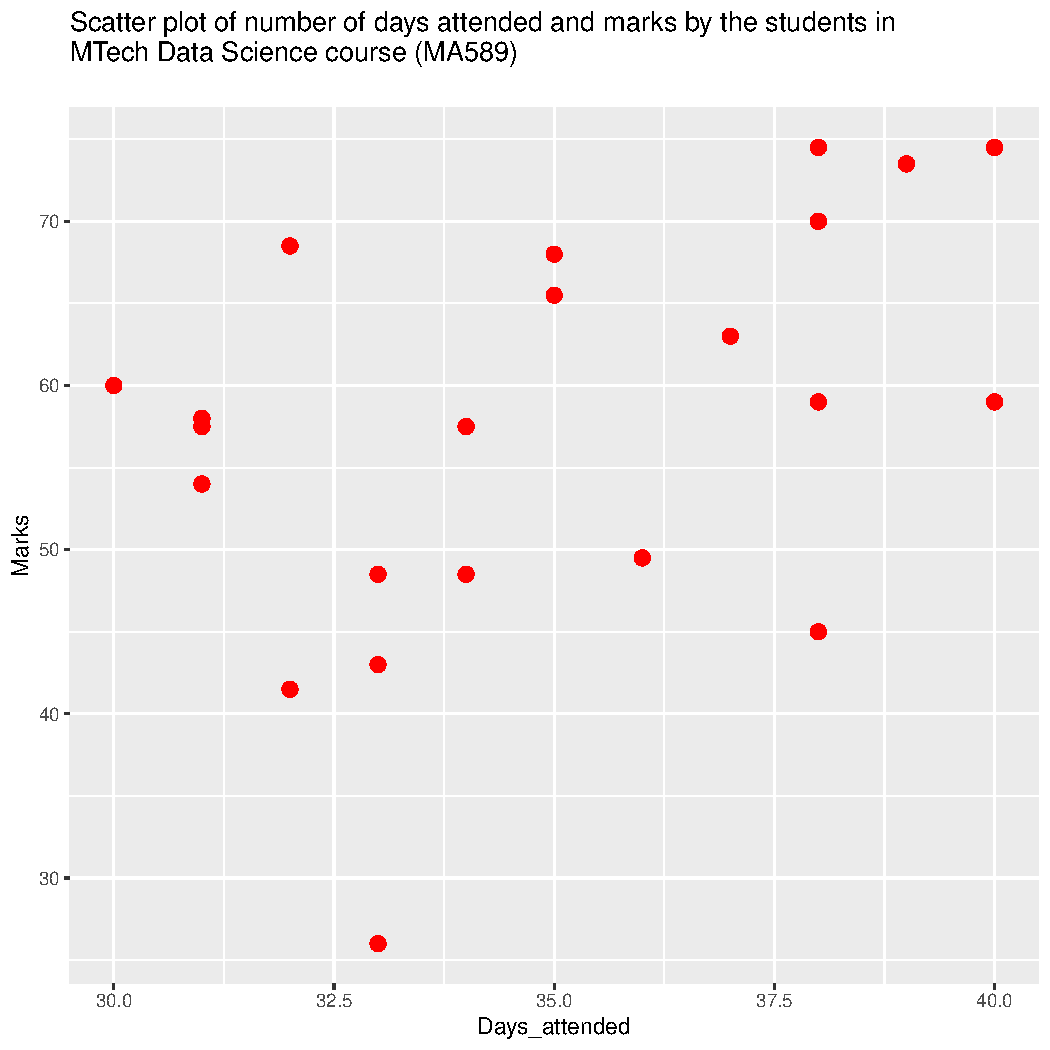
\includegraphics[height=6cm, width=10cm, trim= 0cm 0cm 0cm 2cm]{unnamed-chunk-2-1.pdf} 

	


\end{frame}


\begin{frame}
	\frametitle{ }
	\begin{itemize}
	
	\item We will do a regression analysis to the above data to find the answer. Is using regression appropriate here?
	\vspace{0.5cm}
	
	\item \textbf{Strong Advice:} As a Data Scientist/Statistician, you have to \textbf{spent a lot of your time} and effort to\textbf{ pre-process/clean the raw data} to make it \textbf{analysis ready}. It is part of your job to clean the data: so learn it quickly!!
	\vspace{0.5cm}
	
	
	\item Here is the output after fitting a regression line in R:
\end{itemize}

	
\end{frame}


\begin{frame}
	\frametitle{Fitting Regression line}
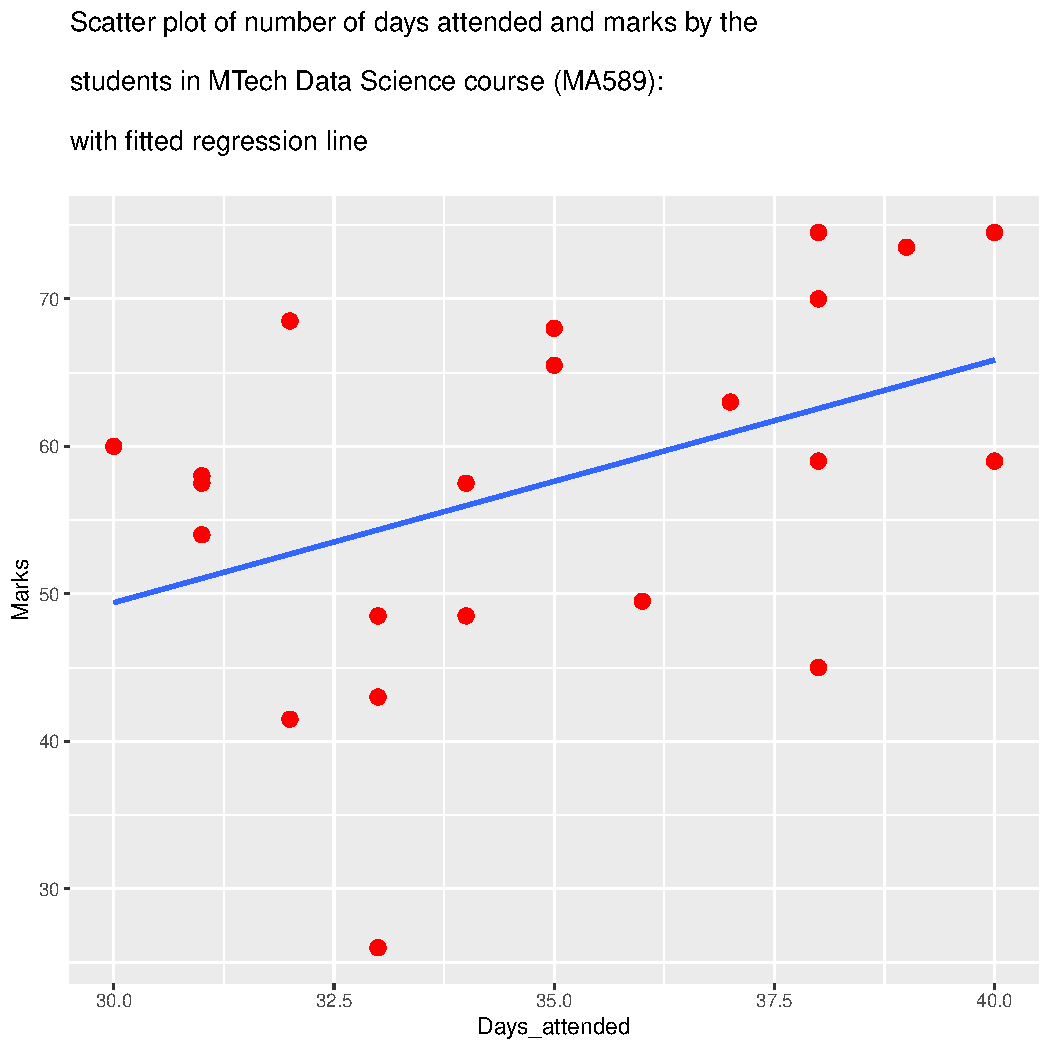
\includegraphics[height=6cm, width=10cm, trim= 0cm 0cm 0cm 2cm]{unnamed-chunk-4-1.pdf}	
	
\end{frame}

% \begin{frame}
% 	\frametitle{Residual Analysis }
% 	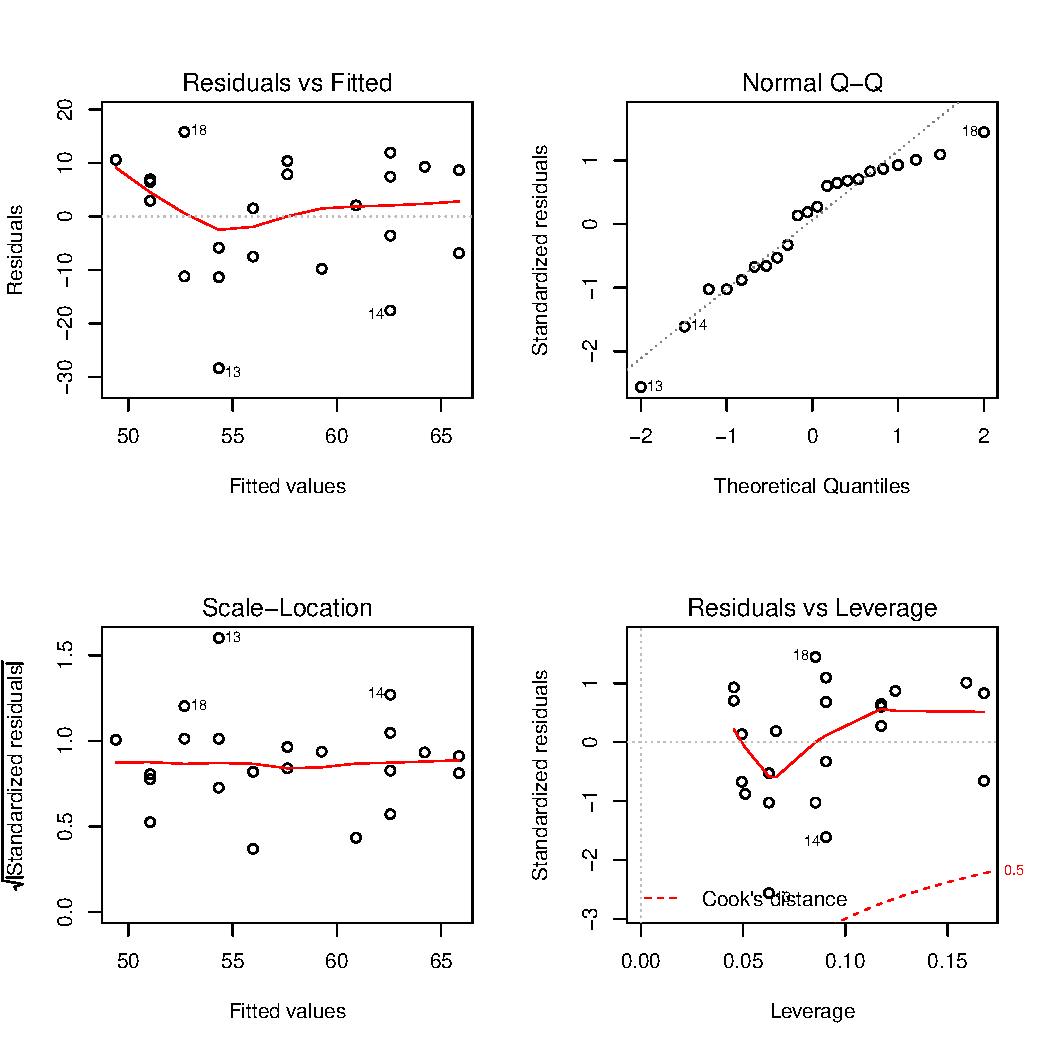
\includegraphics[height=6cm, width=10cm, trim= 0cm 0cm 0cm 2cm]{unnamed-chunk-5-1.pdf}	
% 	
% \end{frame}


\begin{frame}
	\frametitle{Linear Models: Simple and Multiple Linear Regressions}
	
	The regression framework can be characterized in the following way: %\footnote{Handbook of Regression Analysis. By Samprit Chatterjee and Jeffrey S. Simonoff.}:
	\begin{itemize}
		\item We have one particular variable that we are\textbf{ interested in understanding or modeling}, such as sales of a particular product, sale price of a home, or 	voting preference of a particular voter. This variable is called the \textbf{target, response, or dependent variable, and is usually represented} by $y$.
		
		\item We have a set of $p$ \textbf{other variables} that we think might be\textbf{ useful in predicting or modeling the target variable} (the price of the product, the competitor's price, and so on; or the lot size, number of bedrooms, number of bathrooms of the home, and so on; or the gender, age, income, party membership of the voter, and so on). These are called the \textbf{predicting, or independent variables, and are usually represented} by $x_1, x_2, \cdots, x_p$.
		
\end{itemize}	
	
\end{frame}

% == == == == == == == == == == == == == == == == == == == == 
% Frame: Our Aim
\begin{frame}
   \frametitle{Our Aim}
   \begin{itemize}
      \item To build a relationship between $y$ and $x$.
      \item That means to write $y$ as a function of $x$.
      \item Observed data: $(x_i,\,y_i)$ for $i=1,\,2,\,\ldots,\,n$
      \item We want a function of $x$, say $f(\cdot)$, such that
         \begin{align*}
            \sum_{i=1}^{n} \left( y_i - f(x_i) \right)^2
         \end{align*}
         is as small as possible.
      \item There are infinite solutions for this problem.
      \item Therefore, we want to impose constraint the set of functions over
         which the minimization is performed.
   \end{itemize}
\end{frame}


\begin{frame}
%	\frametitle{ }
	\begin{itemize}
		\item Typically, a regression analysis is used for one (or more) of three purposes:
			\vspace{0.5cm}
		
\begin{enumerate}
	\item \textbf{modeling the relationship} between $x$ and $y$;
	\vspace{0.5cm}
	
	\item \textbf{prediction of the target} variable (forecasting);
		\vspace{0.5cm}
	
	\item  and \textbf{testing of hypotheses}.
\end{enumerate}
\end{itemize}	
	
\end{frame}

\begin{frame}
\frametitle{Linear Models: Meaning of Linearity}% and Transformation} 


\textbf{What does ``Linear'' mean?}
\begin{itemize}
	\item A linear model is \textbf{linear in the parameters $\beta$, but not necessarily in the $x$'s,} e.g.
	\bigskip
	\begin{itemize}
		\item[*] $y=\beta_0 + \beta_1x +\beta_2x^2$ is a \textbf{linear model}, because it is linear in $\beta$ (even though not in $x$).
		\bigskip
		\item[*] $y=\beta_0 + \beta_1x^{\beta_2}$ is a \textbf{non-linear model,} because it is not linear in $\beta$.
		
	\end{itemize}
\end{itemize}




\textbf{Transformation}
\begin{itemize}
	\item Clearly $y=f(x) = \beta_0x^{\beta_1}$ is \textbf{not a linear model,} but
	$$\ln f(x) = \ln \beta_0 + \beta_1\ln x$$
	If we let $f^* = \ln f , \beta_0^* = \ln \beta_0, \beta_1^* = \beta_1, x^* = \ln x$,
	we have
	$$f^* = \beta_0^* + \beta_1^*x^*,$$
	which is \textbf{a linear model.}

\end{itemize}






\end{frame}


\begin{frame}
\frametitle{Transformation}

\begin{itemize}

	\item Thus, although linear models seem to be simple and restrictive, they \textbf{can actually be quite flexible by transformation of the response and the predictors.}
	\bigskip
	\item Linear models are \textbf{not just straight lines, they can be curved.} Can you give an examples?
\end{itemize}
		\vspace{0.5cm}
		
	Transform the following \textbf{non-linear models to linear models:}
	\vspace{0.25cm}
	\begin{itemize}
		\item $y = \frac{e^{\beta x}}{1 + e^{\beta x}}$, where $y \in (0,1)$.
		\vspace{0.5cm}
		
		\item $y = \frac{1}{\beta_0 + \beta_1x_1 + \beta_2x_2}\cdot $
		
		% \item $y = e^{e^{\beta x}} -1$, where $y > 0$.
	\end{itemize}	

\end{frame}


% == == == == == == == == == == == == == == == == == == == ==


\begin{frame}
	\frametitle{Simple Linear Regression}
	\begin{itemize}
		\item Just one predictor $x$, i.e. $p=1$, where $p$ indicates the number of predictors in a multiple linear regression model. 
		\vspace{0.5cm}
		
		\item The model for the \textbf{simple linear regression} is given by
		\textbf{$$y=\beta_0 + \beta_1x + \epsilon,$$} where $y$ is the \textbf{outcome} variable (random), $x$ is the \textbf{independent/predictor} variable (non-random) and $\epsilon$ is the \textbf{random error term}. $\beta_0$ (intercept) and $\beta_1$ (slope) are model parameters (unknown constants). 
		\vspace{0.5cm}
		
		\item Equivalently, the \textbf{model can be written} for $i=1,2,\cdots, n$ number of observations $(x_1, y_1), \cdots, (x_n, y_n)$ as
		$$y_i = \beta_0 + \beta_1x_i + \epsilon_i, i = 1,\ldots,n.$$
		\vspace{0.01cm}
		
		\item How do you \textbf{interpret} $\beta_0$ (intercept) and $\beta_1$ (slope)?
	\end{itemize}
\end{frame}

\begin{frame}
   \frametitle{Assumptions: }
   \begin{enumerate}

      \item The \textbf{expected value of the errors is zero}: $E(\epsilon_{i}) = 0$ for all $i$ 
         \vspace{0.5cm}



      \item The \textbf{variance of the error is constant}
         (\emph{homoscedasticity}): $Var(\epsilon_i)=\sigma^2$ for all
         $i$
         \vspace{0.5cm}
      \item The \textbf{errors} ($\epsilon_i$) are \textbf{uncorrelated} with
         each other: $Cov(\epsilon_i,\, \epsilon_j) = 0$ for all $i\neq j$
         % 				
         % 	 \textbf{$Var(Y|X=x)=\sigma^2$}
         % 			\vspace{0.5cm}

         % \item Errors ($\epsilon_i$) are \textbf{normally distributed}

   \end{enumerate}	
   % 			\vspace{0.5cm}
   %
   % \begin{itemize}
   % 	\item The first three assumptions are required to estimate the model parameters. They mean: 	\\
   % 	The \textbf{\emph{errors} $\epsilon_i$'s are uncorrelated} with
   % 	\begin{eqnarray*}
   % 		E(\epsilon_i|x_i) &=& E(\epsilon_i)=0,i=1,\ldots,n\\
   % 		Var(\epsilon_i|x_i) &=& Var(\epsilon_i)=\sigma^2, i=1,\ldots,n
   % 	\end{eqnarray*}
   % \end{itemize}		
\end{frame}



\begin{frame}
	\frametitle{Assumptions: What they means? }

\begin{enumerate}
	\item The \textbf{errors} ($\epsilon_i$) are \textbf{uncorrelated} with each other. This violation most often occurs in data that are ordered in time (time series data), where errors that are near each other in time are often similar to each other (such time-related correlation is called autocorrelation). \textbf{Violation of this assumption} can lead to very \textbf{misleading assessments} of the strength of the regression.
			\vspace{0.5cm}	
	\item The \textbf{expected value of the errors is zero} ($E(\epsilon_{i}) = 0$ for all $i$). That is, it cannot be true that for certain observations the model is systematically too low, while for others it is systematically too high.
			\vspace{0.5cm}	
	
	\item 	The assumption of \emph{\textbf{homoscedasticity (constant variance)}}: each outcome observation ($Y$) has exact same variance (also for error). If $Y$ follows Poisson distribution, this assumption is violated. Why?
			% \vspace{0.5cm}
	
	
	% \item The \textbf{assumption of \emph{normality} of errors is NOT necessary for estimation}; however it is \textbf{necessary for inference} (e.g. testing of hypothesis, confidence intervals).
	
\end{enumerate}

\end{frame}


\begin{frame}
	\frametitle{Least Squares Estimation}
	\begin{itemize}
		\item Goal: To \textbf{estimate $\beta_0,\beta_1$ by minimizing error} in some sense (e.g. squared error)
		\bigskip
		\item One reasonable way is to use the \textbf{\emph{principle of Least Squares}, i.e. minimize the objective function}
		$$Q(\beta_0,\beta_1) = \sum_{i=1}^n \epsilon_i^2 = \sum_{i=1}^n (y_i - \beta_0 - \beta_1x_i)^2$$
		with respect to $\beta_0,\beta_1$.
	\end{itemize}
	
	
	\begin{itemize}
		\item \textbf{Differentiate} $Q(\beta_0,\beta_1)$ with respect to $\beta_0,\beta_1$ and \textbf{equate the partial derivatives to zero} to get the estimates $\hat\beta_0,\hat\beta_1$.
		\bigskip
		\item The resulting equations are called \textbf{\emph{normal equations}:}
		\begin{eqnarray*}
			\sum_{i=1}^n (y_i - \beta_0 - \beta_1x_i) = 0 \\
			\sum_{i=1}^n x_i(y_i - \beta_0 - \beta_1x_i) = 0
		\end{eqnarray*}
	\end{itemize}
		
	
\end{frame}


\begin{frame}
	\frametitle{Least Squares Estimation}
	\begin{itemize}
		\item The \textbf{solution is given by}
		\begin{eqnarray*}
			\hat\beta_0 = \bar y - \hat\beta_1\bar x \\
			\hat\beta_1 = S_{xy}/S_{xx}
		\end{eqnarray*}
		where
		$$S_{xx} = \sum_{i=1}^n (x_i - \bar x)^2\; \textrm{and}\; S_{xy} = \sum_{i=1}^n (x_i - \bar x)(y_i - \bar y).$$
		\item $\hat\beta_0$ and $\hat\beta_1$ are called the \textbf{least squares estimator (LSE)} of $\beta_0$ and $\beta_1$ respectively.
	\end{itemize}	
	
\end{frame}


\begin{frame}
   \frametitle{Properties of $\hat\beta_0$ and $\hat\beta_1$ }
   \begin{itemize}
      \item $\hat\beta_0$ and $\hat\beta_1$ are linear combination of $y_i$'s. 
         \vspace{0.5cm}	

      \item $\hat\beta_0$ and $\hat\beta_1$ are unbiased for $\beta_0$ and $\beta_1$, respectively. 
         \vspace{0.5cm}	

      \item Variances of $\hat\beta_0$ and $\hat\beta_1$ are 
         \begin{eqnarray*}
            Var(\hat\beta_0) &=& \sigma^2\Big(\frac{1}{n}+\frac{\bar x^2}{S_{xx}}\Big) \\
            Var(\hat\beta_1) &=& \frac{\sigma^2}{S_{xx}}
         \end{eqnarray*}
   \end{itemize}
\end{frame}

%
% \begin{frame}
%    %	\frametitle{ }
%    \begin{itemize}
%       \item  Do the least square based estimation problem different from the
%          likelihood based estimation procedure?
%          \vspace{0.5cm}	
%       \item \textbf{Geometrically} speaking, \textbf{minimizing} $\sum_{i=1}^n
%          (y_i - \beta_0 - \beta_1x_i)^2$ this is \textbf{equivalent to
%          minimizing the sum of squared vertical distances} between the actual
%          $y$-values and any regression line to be fitted.
%          \bigskip
%    \end{itemize}	
% \end{frame}

\begin{frame}
   \frametitle{Linear Estimator }
   \begin{defn}[\textbf{Linear Estimator}]
      An estimator $\hat\theta$ is called linear estimator of $\theta$ if
      $\hat\theta$ is a \textbf{linear combination} of random observations. 
   \end{defn}
   \vspace{0.5cm}

   \begin{defn}[\textbf{BLUE}]
      An estimator $\hat\theta$ is called the best linear unbiased estimator
      (\textbf{BLUE}) of $\theta$ if $\hat\theta$ is \textbf{linear and unbiased
      estimator} of $\theta$ and $\hat\theta$ has \textbf{minimum variance
      among} all linear unbiased estimator of $\theta$. 
   \end{defn}

\end{frame}


\begin{frame}
   \frametitle{Gauss-Markov Theorem (Without proof)}
   \begin{theorem}
      If the model assumptions hold true, the LSEs $\hat\beta_0$ and
      $\hat\beta_1$ are BLUE of $\beta_0$ and $\beta_1$, respectively. 
   \end{theorem}
\end{frame}

\begin{frame}
   \frametitle{A Few Definitions}
   \begin{itemize}
      \item \emph{\textbf{Fitted values}}: $\hat y_i = \hat\beta_0 + \hat\beta_1x_i,\; i=1,\ldots,n$
         \bigskip
      \item \emph{\textbf{Residuals}}: Difference between observed and
         fitted values of $y$, i.e. $$e_i = y_i - \hat y_i,\; i=1,\ldots,n$$
      \item The objective function evaluated at the LSE, i.e.
         $Q(\hat\beta_0,\hat\beta_1)$ is called the \textbf{\emph{residual sum
         of squares} ($SS_{Res}$).}

         $$SS_{Res} = \sum_{i=1}^n (y_i - \hat\beta_0 - \hat\beta_1x_i)^2 =
         \sum_{i=1}^{n} \left( y_i - \widehat{y}_i \right)^2 = \sum_{i=1}^{n}
         e_i^2$$

   \end{itemize}
\end{frame}

%
\begin{frame}
   \frametitle{Properties of Least Squares Fit:}
   \begin{enumerate}
      \item $\sum_{i=1}^{n}e_i = 0.$ (from the first normal equation)
         \vspace{0.5cm}

      \item $\sum_{i=1}^{n} y_i = \sum_{i=1}^{n} \hat y_i$. (using (1))
         \vspace{0.5cm}

      \item $\sum_{i=1}^{n} x_i e_i = 0.$ (from the second normal equation)
         \vspace{0.5cm}

      \item $\sum_{i=1}^{n}  \hat y_i e_i = 0.$ (using (1) and (3))
   \end{enumerate}	

\end{frame}


\begin{frame}
\frametitle{Estimation of Error Variance}
\begin{itemize}
   \item It can be shown that 
      $$E(SS_{Res}) = (n-2) \sigma^2$$
      \vspace{0.01cm}

   \item Hence, $\hat\sigma^2 = \frac{SS_{Res}}{n-2} = MS_{Res}$ is an unbiased
      estimator of $\sigma^2$. Here $MS_{Res}$ is residual mean square. 
      \vspace{0.25cm}

   \item Observed value of $\hat\sigma^2 = \frac{SS_{Res}}{n-2}$ is called
      \emph{\textbf{Residual variance}}. It's \textbf{square root is called
      \emph{residual standard error}.}
      \bigskip
   \item Note that $SS_{Res}$ depends on the model. Therefore, any violation of
      model assumptions has serious effect on $\hat\sigma^2$. 
      \vspace{0.25cm}

   \item A convenient computing formula for $SS_{Res}$ is
      $$SS_{Res} = SS_{T} - \hat{\beta_1} S_{xy}, $$ where $$SS_{T} = \sum_{i=1}^{n}(y_i - \bar{y})^2.$$
\end{itemize}	

\end{frame}


% == == == == == == == == == == == == == == == == == == == ==

% == == == == == == == == == == == == == == == == == == == == 
% Frame: Hypothesis Testing
\begin{frame}
   \frametitle{Hypothesis Testing}
   \begin{itemize}
      \item We will talk about mainly following hypotheses:
         \begin{itemize}
            \item $H_0: \beta_1=0$ against $H_1:\beta_1\neq 0$
            \item $H_0: \beta_0=0$ against $H_1:\beta_0\neq 0$
         \end{itemize}
         \bigskip
      \item Assumption: We need the following assumption along with previous
         assumptions.
         \begin{center}
            $\boldsymbol{\epsilon} = \left( \epsilon_1,\,\ldots,\,\epsilon_n
            \right)$ has a $n$-dimensional normal distribution.
         \end{center}
   \end{itemize}
\end{frame}


\begin{frame}
	\frametitle{Hypothesis Testing: $\beta_1$ }
\begin{itemize}
% \item The fourth assumption of linear regression is required for testing of hypothesis: Errors are independent and normally distributed. 
% \vspace{0.2cm}
%
\item Want to test the hypothesis that the \textbf{slope} parameter ($\beta_1$) equals to a constant (a value, say $\beta_{10}$):
$$H_0: \beta_1 = \beta_{10} \mbox{ ag. } H_1: \beta_1 \neq \beta_{10} $$
%\vspace{0.01cm}

\item Note that, $y_i \sim N(\beta_0 + \beta_1 x_i, \sigma^2)$ and $y_i$'s are independent. 
\vspace{0.2cm}

\item $\hat{\beta_1} \sim N(\beta_1, \frac{\sigma^2}{S_{xx}}) \implies z = \frac{\hat{\beta_1} - \beta_1}{\sqrt{\sigma^2/S_{xx}}} \sim N(0, 1)$. But $\sigma$ is unknown. 
\vspace{0.2cm}

\item $\frac{(n-2) MS_{Res}}{\sigma^2} \sim \chi_{n-2}^2$. Also $MS_{Res}$ and $\hat\beta_1$ are independent. 
\vspace{0.2cm}

\item Therefore, the test statistic is 
$$t = \frac{\hat{\beta_1} - \beta_{10}}{\sqrt{MS_{Res}/S_{xx}}} \sim t_{n-2}, \mbox{ under } H_0.  $$
%\vspace{0.1cm}

\item Reject $H_0$ iff $|t| > t_{n-2, \alpha/2};$ (at level $\alpha$). 
\item The test can be performed using $F$-distribution with appropriate degrees
   of freedom.
\end{itemize}	

\end{frame}


\begin{frame}
	\frametitle{Hypothesis Testing: $\beta_0$ }
\begin{itemize}
	
	\item Want to test the hypothesis that the \textbf{intercept} parameter ($\beta_0$) equals to a constant (a value, say $\beta_{00}$):
	$$H_0: \beta_0 = \beta_{00} \mbox{ ag. } H_1: \beta_0 \neq \beta_{00} $$
	%\vspace{0.01cm}
%	
%	\item Note that, $y_i \sim N(\beta_0 + \beta_1 x_i, \sigma^2)$ and $y_i$'s are independent. 
%	\vspace{0.2cm}
	
	\item $\hat{\beta_0} \sim N(\beta_0, \sigma^2(\frac{1}{n} + \frac{\bar{x}^2}{S_{xx}})) \implies z = \frac{\hat{\beta_0} - \beta_0}{\sqrt{\sigma^2(\frac{1}{n} + \frac{\bar{x}^2}{S_{xx}})}} \sim N(0, 1)$. But $\sigma$ is unknown. 
	\vspace{0.2cm}
	
	\item $\frac{(n-2) MS_{Res}}{\sigma^2} \sim \chi_{n-2}^2$. Also $MS_{Res}$ and $\hat\beta_1$ are independent. 
	\vspace{0.2cm}
	
	\item Therefore, the test statistic is 
	$$t = \frac{\hat{\beta_0} - \beta_{00}}{\sqrt{MS_{Res}(\frac{1}{n} + \frac{\bar{x}^2}{S_{xx}})}} \sim t_{n-2}, \mbox{ under } H_0.  $$
	%\vspace{0.1cm}
	
	\item Reject $H_0$ iff $|t| > t_{n-2, \alpha/2};$ (at level $\alpha$). 
\end{itemize}
	
\end{frame}


\begin{frame}
	\frametitle{Interval Estimation: $\beta_0$ and $\beta_1$ }
\begin{itemize}
\item To get the CI for $\beta_0$ and $\beta_1$, the pivots are
$$\frac{\hat{\beta_0} - \beta_{0}}{\sqrt{MS_{Res}(\frac{1}{n} + \frac{\bar{x}^2}{S_{xx}})}}, \mbox{ and } \frac{\hat{\beta_1} - \beta_{1}}{\sqrt{MS_{Res}/S_{xx}}}, \mbox{ respectively.} $$
	\vspace{0.2cm}

\item A $100(1-\alpha)\%$ CI for $\beta_0$ is 
$$\Bigg[\hat{\beta_0} \pm t_{n-2, \alpha/2} \sqrt{MS_{Res}\Big(\frac{1}{n} + \frac{\bar{x}^2}{S_{xx}}\Big)} \Bigg]. $$

	\vspace{0.2cm}

\item A $100(1-\alpha)\%$ CI for $\beta_1$ is 
$$\Bigg[\hat{\beta_1} \pm t_{n-2, \alpha/2} \sqrt{\frac{MS_{Res}}{S_{xx}}} \Bigg]. $$


\end{itemize}	

\end{frame}


\begin{frame}
	\frametitle{Interval Estimation: CI for $\sigma^2$}
\begin{itemize}
\item To get the CI for $\sigma^2$, the pivots is
$$\frac{(n-2) MS_{Res}}{\sigma^2} \sim \chi_{n-2}^2$$
	\vspace{0.2cm}

\item A $100(1-\alpha)\%$ CI for $\sigma^2$ is
$$\Bigg[\frac{(n-2) MS_{Res}}{\chi_{n-2; \alpha/2}^2}, \frac{(n-2) MS_{Res}}{\chi_{n-2; 1 - \alpha/2}^2} \Bigg]. $$
\end{itemize}	
	
\end{frame}


\begin{frame}
	\frametitle{Interval Estimation: CI for mean response}
\begin{itemize}
\item A regression model can be used to \textbf{estimate the mean response} $E(y)$ for a particular value of the regressor variable $x$. Let $x_0$ be a value of the regressor variable (must be with the range of original data on $x$). Then $E(y|x_0) = \beta_0 + \beta_1 x_0$.
	\vspace{0.2cm}

\item Then, $\widehat{y_0} = \widehat{E(y|x_0)} = \hat\beta_0 + \hat\beta_1 x_0$

	\vspace{0.2cm}

\item And, $\widehat{y_0}  \sim N\Big(\beta_0 + \beta_1 x_0, \sigma^2\Big(\frac{1}{n} + \frac{(x_0 -\bar{x})^2}{S_{xx}}\Big)\Big) $

	\vspace{0.2cm}

\item Pivot: $\frac{\widehat{y_0} - (\beta_0 + \beta_1 x_0)}{\sqrt{MS_{Res}\Big(\frac{1}{n} + \frac{(x_0 -\bar{x})^2}{S_{xx}}\Big)}} \sim t_{n-2}$
	\vspace{0.2cm}

\item A $100(1-\alpha)\%$ CI for $\beta_0 + \beta_1 x_0$ is
$$\Bigg[\widehat{y_0} \pm t_{n-2; \alpha/2} \sqrt{MS_{Res}\Big(\frac{1}{n} + \frac{(x_0 -\bar{x})^2}{S_{xx}}\Big)} \Bigg].$$
\end{itemize}	
	
\end{frame}


\begin{frame}
	\frametitle{Prediction Interval for New Observation:  }
\begin{itemize}
\item Let $x_0$ be a value of the regressor variable (must be with the range of original data on $x$).
	\vspace{0.2cm}

\item The true value of the response is $y_0$ (corresponding to $x_0$). 

	\vspace{0.2cm}

\item We want to provide an interval $I$ such that $P(y_0 \in I) = 1 -\alpha$

	\vspace{0.2cm}

\item Note that the point estimate of $y_0$ is $\hat y_0 = \hat\beta_0 + \hat\beta_1 x_0$.

	\vspace{0.2cm}

\item Consider $ \psi = y_0 - \hat y_0$. 

	\vspace{0.2cm}

\item Then, $E(\psi) = 0, Var(\psi) =  \sigma^2\Big(1 + \frac{1}{n} + \frac{(x_0 -\bar{x})^2}{S_{xx}}\Big)$
\vspace{0.2cm}

\item $\psi \sim N \Bigg(0, \sigma^2\Big(1 + \frac{1}{n} + \frac{(x_0 -\bar{x})^2}{S_{xx}}\Big)  \Bigg)$

\vspace{0.2cm}

\item Pivot: $\frac{y_0 - \hat y_0}{\sqrt{MS_{Res}\Big(1 + \frac{1}{n} + \frac{(x_0 -\bar{x})^2}{S_{xx}}\Big)}} \sim t_{n-2} $
\end{itemize}	
	
\end{frame}


\begin{frame}
	\frametitle{Prediction Interval for New Observation:  }
\begin{itemize}
\item A $100(1-\alpha)\%$ prediction interval is
$$\Bigg[\hat y_0 \pm t_{n-2; \alpha/2} \sqrt{MS_{Res}\Big(1 + \frac{1}{n} + \frac{(x_0 -\bar{x})^2}{S_{xx}}\Big)}  \Bigg]. $$
\end{itemize}	
	
\end{frame}

\begin{frame}
	\frametitle{Coefficient of determination: $R^2$ }
\begin{itemize}
		\item \emph{\textbf{Coefficient of determination:}}
$$R^2 = \frac{SS_{Reg}}{SS_{T}}  = 1 - \frac{SS_{Res}}{SS_{T}} = 1 - \frac{\sum_i (y_i - \hat y_i)^2}{\sum_i (y_i - \bar y)^2},$$
where $SS_{Reg} = \sum_i (\hat y_i - \bar y)^2$

%\vspace{0.2cm}
%
%\item Also called \emph{multiple correlation coefficient} in the context of multiple linear regression
\vspace{0.25cm}
\item It is a bounded quantity: \textbf{$0\le R^2 \le 1$}

\vspace{0.2cm}
		\item  $R^2$ is interpreted as the \textbf{``proportion of variation explained by the model''.}

\vspace{0.2cm}
\item \textbf{Higher values of $R^2$ are desirable} ($R^2$ close to 1 indicates a good fit), but ``how high is high'' \textbf{depends on the context.}
		\vspace{0.25cm}

\end{itemize}	
	
\end{frame}


% \begin{frame}
% 	\frametitle{$F$-Test for Regression }
% \begin{itemize}
% 	\item Large value of the sum of squares for regression $SS_{Reg} = SS_{T} - SS_{Res}$ indicates the simple regression
% 	mean function $E(Y |X = x) = \beta_0 + \beta_1 x$ should be a \textbf{significant improvement over the mean function} $E(y|X = x) = \beta_0$.
% 	\vspace{0.5cm}
% 	\item This is equivalent to saying
% 	that the \textbf{additional parameter} ($\beta_1$) in the simple regression mean function is \textbf{non-zero}. In other words, that $E(Y |X = x)$ is not constant with respect to $X$.
% 	\vspace{0.5cm}
% 	\item To test $$H_0: E(Y |X = x) = \beta_0 \mbox{ ag. } H_1: E(Y |X = x) = \beta_0 + \beta_1 x $$
% %		\vspace{0.5cm}
% 	\item Test statistics is a ratio, defined as F :
% 	$$ F = \frac{SS_{Reg}/1}{\hat\sigma^2} = \frac{SS_{Reg}/1}{SS_{Res}/(n-2)} \sim F_{1, n-2} $$
% \end{itemize}	
% 	
% \end{frame}



\begin{frame}
	\frametitle{Simple Linear Regression in Heights Data }
\textbf{Heights Data Example}
\begin{itemize}
	\item Aim: To study inheritance of height from generation to generation
      (among females)
	\item Data on heights of $n=1375$ mothers in the UK under the age of 65 and
      one of their adult daughters over the age of 18.
   \item Collected and organized during the period 1893--1898 by the famous
      statistician Karl Pearson.
   \item The dataset is publicly available 
      \begin{itemize}
         \item R-packages: alr4, UsingR
         \item GitHub:
            \url{https://github.com/kbroman/PearsonData/blob/master/mother_daughter.csv}
      \end{itemize}
	% \item A historical use of regression to study inheritance of height from
      % generation to generation
   \item Sample correlation coefficient is 0.491
\end{itemize}		
\end{frame}


% \begin{frame}
% 	%\frametitle{What do you see?}
% 	\begin{figure}
% 		\begin{center}
% 			\scalebox{0.4}[0.4]{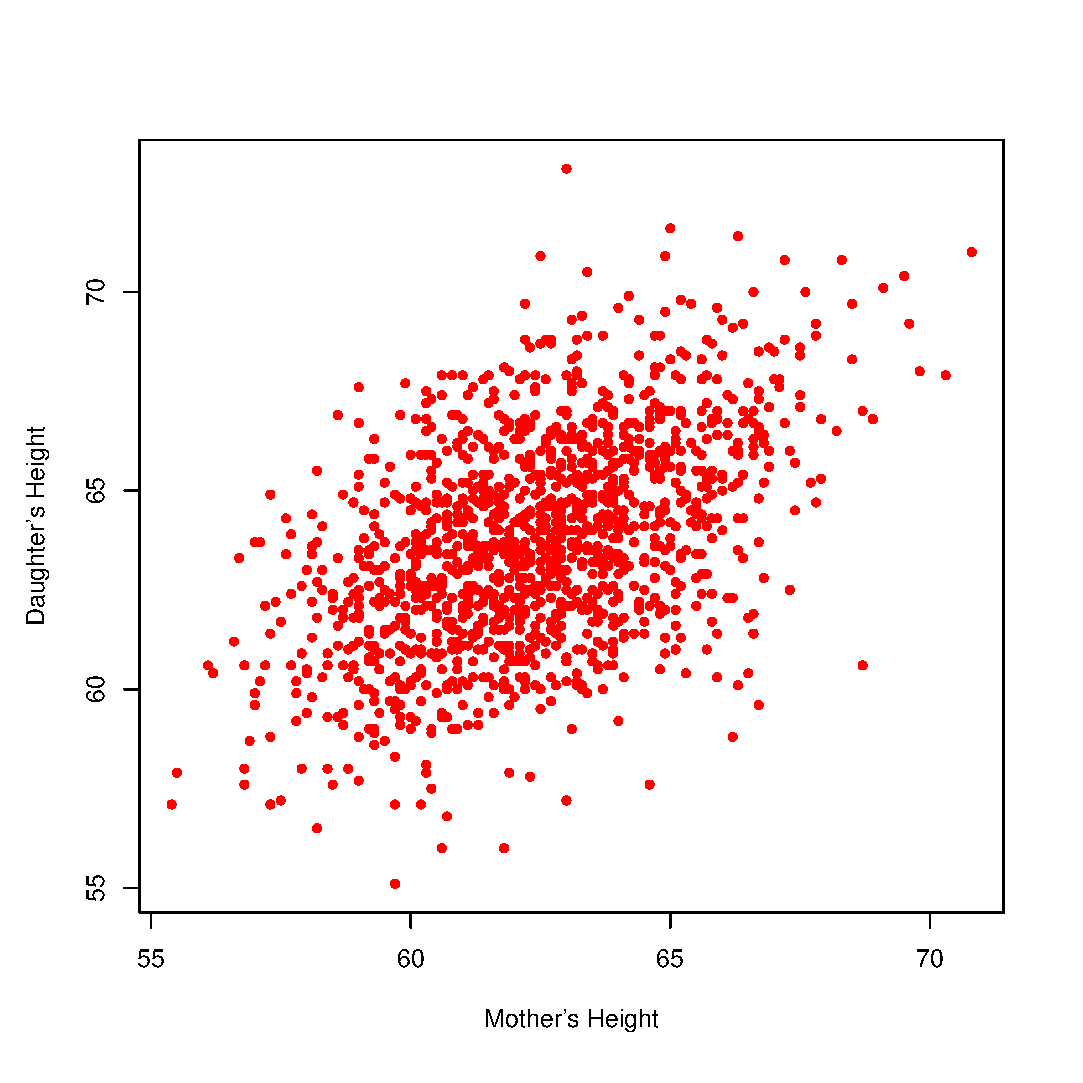
\includegraphics{scatterplot1.eps}}
% 		\end{center}
% 	\end{figure}
% \end{frame}


\begin{frame}[fragile]
	\frametitle{Simple Linear Regression: Using R}
	\begin{verbatim}
	> height.lm <- lm(Dheight~Mheight,data=heights)
	> summary(height.lm)
	...
	Coefficients:
	             Estimate  Std.Error  t-value Pr(>|t|)
	(Intercept) 29.91744    1.62247   18.44   <2e-16 ***
	Mheight      0.54175    0.02596   20.87   <2e-16 ***
	---
	Signif. codes:  0 *** 0.001 ** 0.01 * 0.05 . 0.1  1

	Residual standard error: 2.266 on 1373 degrees of
	freedom Multiple R-squared: 0.2408, 
	adjusted R-squared: 0.2402
	F-statistic: 435.5 on 1 and 1373 DF,  
	p-value: < 2.2e-16

	\end{verbatim}
\end{frame}

% \begin{frame}[fragile]
% 	\frametitle{Let's look at the Regression Line}
% 	\begin{verbatim}
% 	> plot(Dheight ~ Mheight, heights, 
% 	xlab="Mother's Height", ylab="Daughter's Height",
% 	pch=20, col=2)
%
% 	> abline(coef(height.lm), lty=5, col=4)
%
% 	> abline(0,1)
% 	\end{verbatim}
% \end{frame}

\begin{frame}
	\begin{figure}
		\begin{center}
			\scalebox{0.4}[0.4]{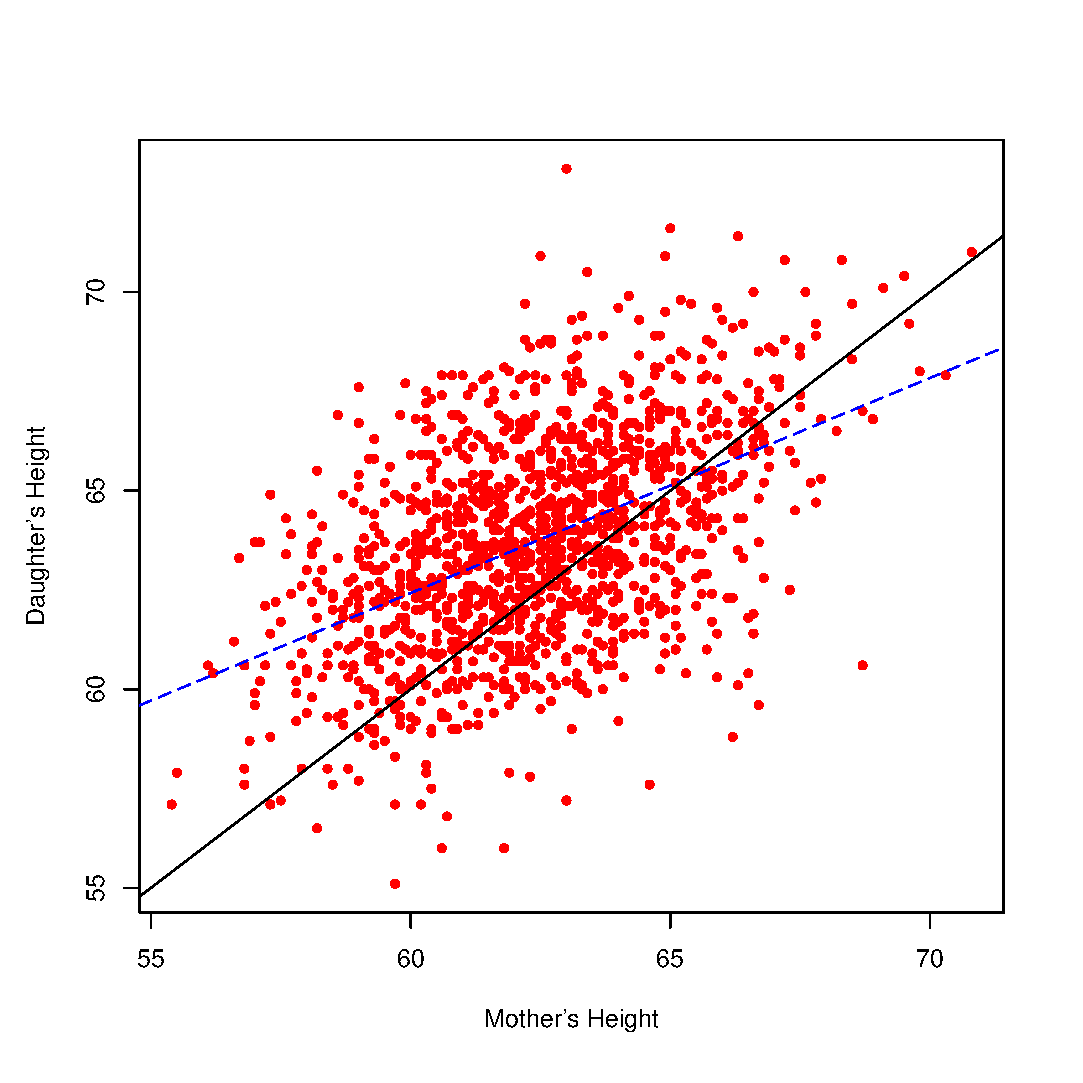
\includegraphics{regline1.eps}}
		\end{center}
	\end{figure}
\end{frame}

\begin{frame}
	\frametitle{Regression Effect}
	\begin{itemize}
      \item It's an empirical phenomenon, also called
         \textcolor{red}{``regression to the mean''} or \textcolor{red}{``regression to
         mediocrity'',} e.g.
		\bigskip
		\begin{itemize}
         \item Daughters of tall mothers \textcolor{red}{tend to be tall, but
            not as tall} as their mothers; daughters of short mothers tend to be
            short, but not as short as their mothers (same trend between sons
            and fathers)
			\bigskip
         \item Students \textcolor{red}{doing well in Mid-term tend to do well
            in the Final, but not as well} as the Mid-term; students doing
            poorly in Mid-term tend to do poorly in the Final, but not as poorly
            as the Mid-term!
		\end{itemize}
	\end{itemize}
\end{frame}

% == == == == == == == == == == == == == == == == == == == == 
% Frame: Caution
\begin{frame}
   \frametitle{Caution}
   \begin{itemize}
      \item Do you think a moderate or high absolute value of correlation
         coefficient makes a data ideal for LR?
         \pause
      \item Consider datasets given in next slide.
   \end{itemize}
\end{frame}

% == == == == == == == == == == == == == == == == == == == == 
% Frame: 
\begin{frame}
   \frametitle{Anscombe's Examples (1973)}
   \begin{table}[ht]\scriptsize
      \centering
      \begin{tabular}{c@{\hspace{2mm}}cc@{\hspace{2mm}}cc@{\hspace{2mm}}cc@{\hspace{2mm}}c}
         \toprule
         \multicolumn{2}{c}{Dataset 1} &
         \multicolumn{2}{c}{Dataset 2} &
         \multicolumn{2}{c}{Dataset 3} &
         \multicolumn{2}{c}{Dataset 4} \\
         \cmidrule(lr){1-2}
         \cmidrule(lr){3-4}
         \cmidrule(lr){5-6}
         \cmidrule(lr){7-8}
         $x$ & $y$ & $x$ & $y$ & $x$ & $y$ & $x$ & $y$ \\ 
         \midrule
         10.00 & 8.04 & 10.00 & 9.14 & 10.00 & 7.46 & 8.00 & 6.58 \\ 
         8.00 & 6.95 & 8.00 & 8.14 & 8.00 & 6.77 & 8.00 & 5.76 \\ 
         13.00 & 7.58 & 13.00 & 8.74 & 13.00 & 12.74 & 8.00 & 7.71 \\ 
         9.00 & 8.81 & 9.00 & 8.77 & 9.00 & 7.11 & 8.00 & 8.84 \\ 
         11.00 & 8.33 & 11.00 & 9.26 & 11.00 & 7.81 & 8.00 & 8.47 \\ 
         14.00 & 9.96 & 14.00 & 8.10 & 14.00 & 8.84 & 8.00 & 7.04 \\ 
         6.00 & 7.24 & 6.00 & 6.13 & 6.00 & 6.08 & 8.00 & 5.25 \\ 
         4.00 & 4.26 & 4.00 & 3.10 & 4.00 & 5.39 & 19.00 & 12.50 \\ 
         12.00 & 10.84 & 12.00 & 9.13 & 12.00 & 8.15 & 8.00 & 5.56 \\ 
         7.00 & 4.82 & 7.00 & 7.26 & 7.00 & 6.42 & 8.00 & 7.91 \\ 
         5.00 & 5.68 & 5.00 & 4.74 & 5.00 & 5.73 & 8.00 & 6.89 \\ 
         \bottomrule
      \end{tabular}
   \end{table}
\end{frame}

\begin{frame}
    \frametitle{Means \& Standard Deviations}
    \begin{table}\scriptsize
        \centering
        \begin{tabular}{cccccc}
            \toprule
            & & \multicolumn{2}{c}{$x$} & \multicolumn{2}{c}{$y$} \\
            \cmidrule(lr){3-4} \cmidrule(lr){5-6}
            Data Set & N & Mean & SD & Mean & SD \\
            \midrule
            1 & 11 & 7.50 & 2.03 & 9.00 & 3.32 \\
            2 & 11 & 7.50 & 2.03 & 9.00 & 3.32 \\
            3 & 11 & 7.50 & 2.03 & 9.00 & 3.32 \\
            4 & 11 & 7.50 & 2.03 & 9.00 & 3.32 \\
            \bottomrule
        \end{tabular}
    \end{table}
    
    \vspace{0.5cm}
    \begin{center}
       The means and SDs for the 4 data sets are identical to two decimals.
    \end{center}
\end{frame}

\begin{frame}
    \frametitle{Correlations between $x$ and $y$}
    \begin{table}\scriptsize
        \centering
        \begin{tabular}{cccc}
            \toprule
            Data Set & Pearson r & R-squared & Adj. R-sq\\
            \midrule
            1 & 0.82 & 0.67 & 0.63 \\
            2 & 0.82 & 0.67 & 0.63 \\
            3 & 0.82 & 0.67 & 0.63 \\
            4 & 0.82 & 0.67 & 0.63 \\
            \bottomrule
        \end{tabular}
    \end{table}
    
    \vspace{0.5cm}
    \begin{center}
        Correlations, R-squared, adjusted R-squared, are all identical to two decimals.
    \end{center}
\end{frame}

\begin{frame}
    \frametitle{ANOVA Summary Tables}
    \scriptsize
    \begin{table}\scriptsize
        \centering
        \begin{tabular}{c@{\hspace{7mm}}l@{\hspace{7mm}}c@{\hspace{7mm}}c@{\hspace{7mm}}r@{\hspace{7mm}}c@{\hspace{7mm}}c}
            \toprule
            Data Set & Source & $SS$ & $df$ & $MS$ & $F$ & $p$-value \\
            \midrule
            \multirow{3}{*}{1} & Regression & 27.490 & 1 & 27.490 & 18.003 & 0.002 \\
            & Residual & 13.742 & 9 & 1.527 & & \\
            & Total & 41.232 & 10 & & & \\
            \midrule
            \multirow{3}{*}{2} & Regression & 27.470 & 1 & 27.470 & 17.972 & 0.002 \\
            & Residual & 13.756 & 9 & 1.528 & & \\
            & Total & 41.226 & 10 & & & \\
            \midrule
            \multirow{3}{*}{3} & Regression & 27.500 & 1 & 27.500 & 17.966 & 0.002 \\
            & Residual & 13.776 & 9 & 1.531 & & \\
            & Total & 41.276 & 10 & & & \\
            \midrule
            \multirow{3}{*}{4} & Regression & 27.510 & 1 & 27.510 & 17.990 & 0.002 \\
            & Residual & 13.763 & 9 & 1.529 & & \\
            & Total & 41.273 & 10 & & & \\
            \bottomrule
        \end{tabular}
    \end{table}
\end{frame}

\begin{frame}
    \frametitle{The Regression Coefficients}
    \scriptsize
    \begin{table}\scriptsize
        \centering
        \begin{tabular}{@{\hspace{2mm}}c@{\hspace{7mm}}l@{\hspace{7mm}}c@{\hspace{7mm}}c@{\hspace{7mm}}c@{\hspace{7mm}}c@{\hspace{7mm}}c@{\hspace{7mm}}c@{\hspace{2mm}}}
            \toprule
            & & & & & & \multicolumn{2}{c}{95\% CI} \\
            \cmidrule(r){7-8}
            Data Set & & Estimate & $SE$ & $t$ & $p$-value & Lower & Upper \\
            \midrule
            \multirow{2}{*}{1} & Constant & 3.00 & 1.124 & 2.67 & 0.026 & 0.459 & 5.544 \\
            & $x$ & 0.50 & 0.118 & 4.24 & 0.002 & 0.233 & 0.766 \\
            \midrule
            \multirow{2}{*}{2} & Constant & 3.00 & 1.124 & 2.67 & 0.026 & 0.459 & 5.546 \\
            & $x$ & 0.50 & 0.118 & 4.24 & 0.002 & 0.233 & 0.766 \\
            \midrule
            \multirow{2}{*}{3} & Constant & 3.00 & 1.125 & 2.67 & 0.026 & 0.455 & 5.547 \\
            & $x$ & 0.50 & 0.118 & 4.24 & 0.002 & 0.233 & 0.767 \\
            \midrule
            \multirow{2}{*}{4} & Constant & 3.00 & 1.125 & 2.67 & 0.026 & 0.456 & 5.544 \\
            & $x$ & 0.50 & 0.118 & 4.24 & 0.002 & 0.233 & 0.767 \\
            \bottomrule
        \end{tabular}
    \end{table}
    
    \vspace{0.4cm}
    \begin{center}
        \normalsize For all 4 models, $\widehat{y}=0.5x+3$
    \end{center}
\end{frame}

\begin{frame}
    \frametitle{Which dataset is best described by the model?}
    \begin{itemize}
        \item Judging by everything we've just seen, it appears that the models are all equally good
        \vspace{0.3cm}
        \item But if that were true, I wouldn't be doing this talk!
        \vspace{0.3cm}
        % \item It is well known that good graphs are an essential part of data
        %    analysis (Tukey, 1977; Tufte, 1997)
        % \vspace{0.3cm}
        \item Let's look at scatter plots between $x$ and $y$
    \end{itemize}
\end{frame}

\begin{frame}
	\frametitle{ Importance of graphing data before analyzing it}	
	\vspace{0.5cm}

	\begin{center}
		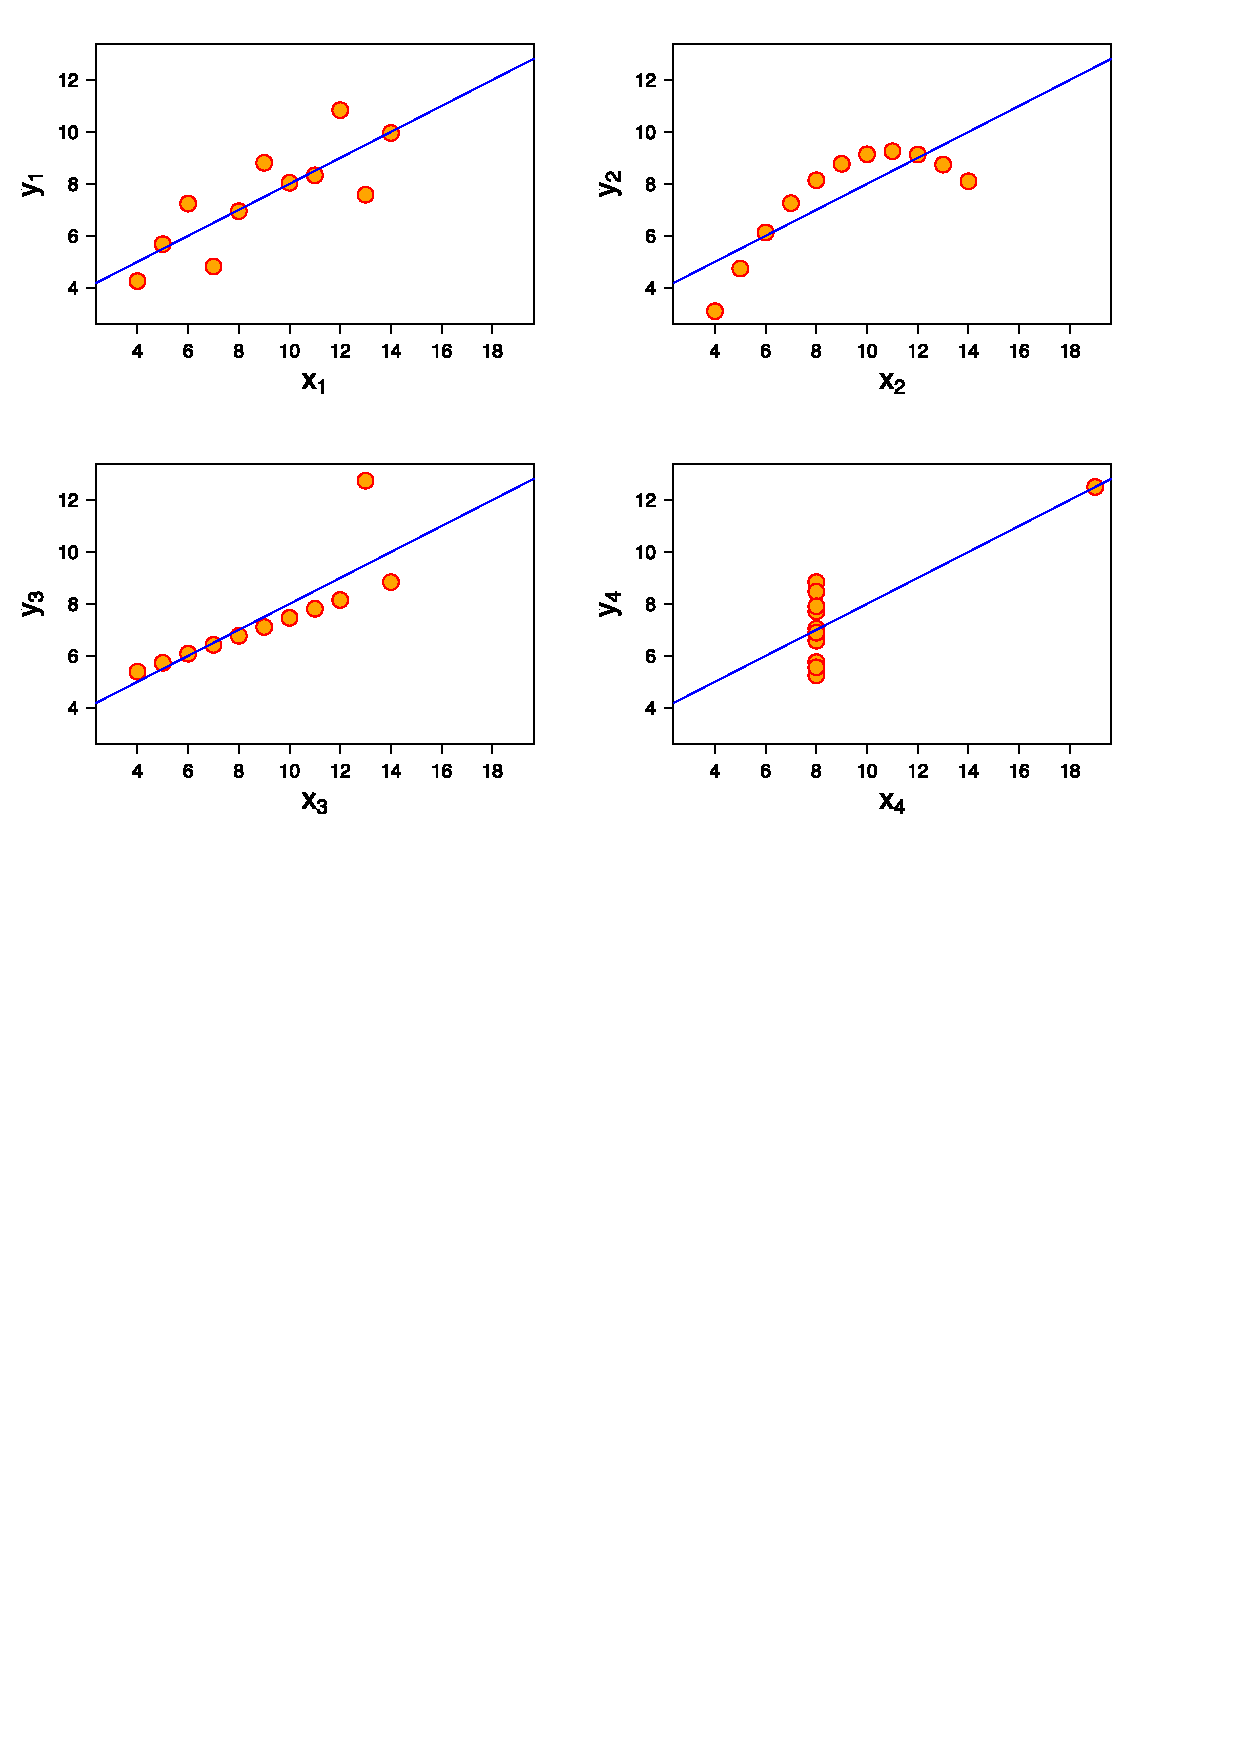
\includegraphics[trim = 0cm 18cm 0cm 1cm, height=6cm]{Anscombe_four_graph.pdf}
	\end{center}

	\vspace{1cm}



\end{frame}

\end{document}
